\documentclass[aspectratio=169]{beamer}

\setbeameroption{show notes on second screen}

\usepackage[utf8]{inputenc}
\usetheme{Madrid}
\usecolortheme{beaver}

\usepackage{graphicx}
\graphicspath{ {./Resources/} }

\title{Project Development Plan}       % Title
\author{Austin, Joe, Matt, Kathryn}                     % Team members
\institute{SNHU/CETA}                                   % Institute
\logo{
\includegraphics[height=0.8cm]{../../AJMK_Logo}}  % Our Logo
\titlegraphic{
\includegraphics[height=2.6cm]{Stencil.png}} % Title graphic

\begin{document}

\frame{\titlepage} % Draw the title page
\note{Hello and thank you for listening, We're team \huge{AKMJ} \normalsize and we're very
excited to present the PDP for our chosen product, the pendulum 328}

\section{Introduction}
\begin{frame}
    \frametitle{Problem Statement}

    \begin{columns}

    \begin{column}{0.4\textwidth}
        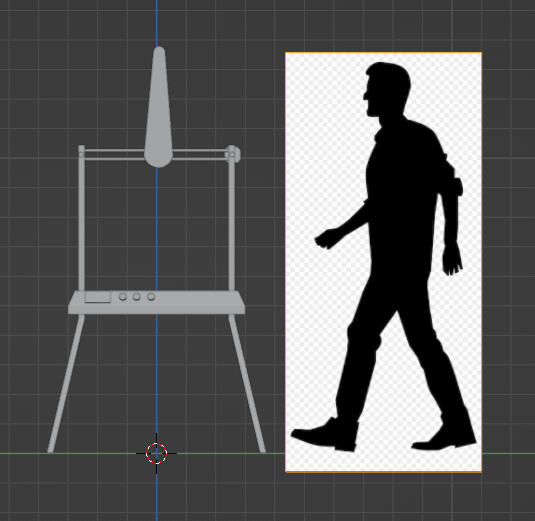
\includegraphics[height=5cm]{Scale}
    \end{column}

    \begin{column}{0.58\textwidth}
        \begin{block}{Our Goal}
        The goal is to make a PID Demonstrator that teaches the operator how to use a PID loop.
        The operator will have control to adjust each individual variable and see how each effects a
        vertical standing pendulum.
    \end{block}
    \end{column}
\end{columns}

\note{
\huge Kat \normalsize

Our goal
\begin{itemize}
 \item Make a PID Demonstrator that teaches the operator how to use a pid loop
 \item control individual variables
 \item balance the pendulum with PID
\end{itemize}
}

\end{frame}

\begin{frame}
    \frametitle{Agenda}

    \begin{columns}
    \begin{column}{0.48\textwidth}
        \setcounter{tocdepth}{1} % Prof requested we do this
        {\tableofcontents}
    \end{column}

    \begin{column}{0.48\textwidth}
        \begin{center}
            
\includegraphics[height=3cm]{../../AJMK_Logo}
            
\includegraphics[height=3cm]{Stencil.png}
        \end{center}
    \end{column}
    \end{columns}

\note{
\huge Everyone \normalsize

\begin{itemize}
 \item We'll do questions at the end
 \item Page numbers are in the bottom right, remember to note what page you'd like us to go back to!
\end{itemize}
}

\end{frame}

\section{Research}
\begin{frame}
    \frametitle{Research}

    There are a few different approaches to the PID demonstrator system.

    \begin{columns}

    \begin{column}{0.48\textwidth}
        \begin{block}{Rotary Inverted Pendulum}
             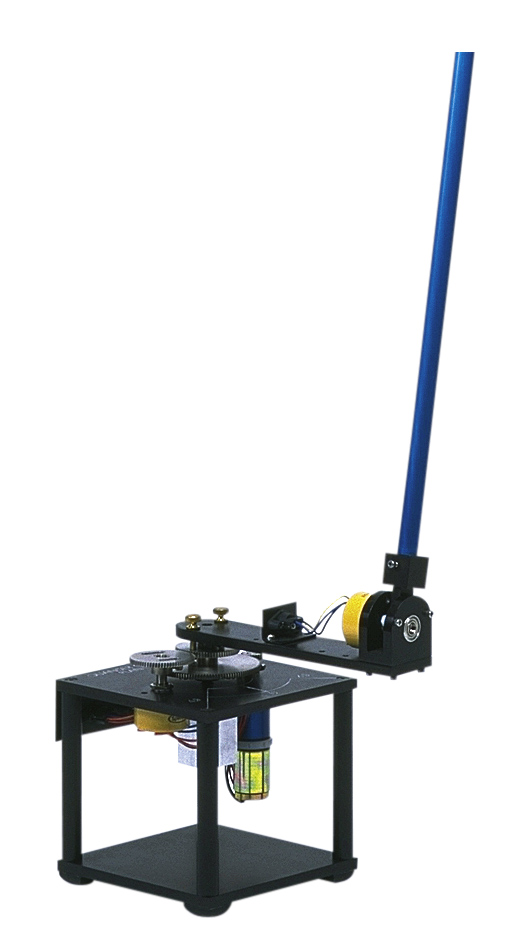
\includegraphics[height=4cm]{RotaryInvertedPendulum}
        \end{block}
        Spins around an axis to produce its motion.
    \end{column}

    \begin{column}{0.48\textwidth}
        \begin{block}{Reaction Wheel Pendulum}
                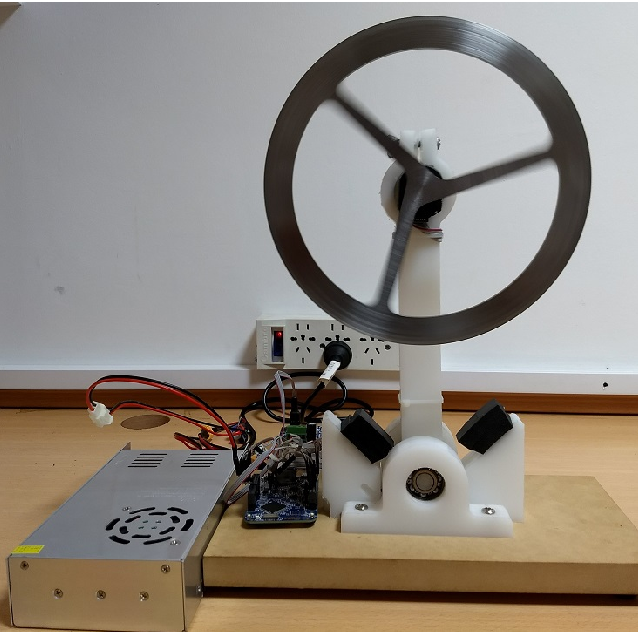
\includegraphics[height=4cm]{ReactionWheel}
        \end{block}
        Uses a reaction wheel to develop a torque against falling over.
    \end{column}
\end{columns}

\note{
\huge Kat and Austin \normalsize

\begin{itemize}
 \item We performed research on other types of pid demonstrator
 \item The rotary inverted pendulum rotates around to create the torque required to balance
 \item A reaction wheel pendulum works like a spacecraft and manufactures a countertorque on the top instead of the bottom
\end{itemize}
}

\end{frame}

\section{ConOps}
\begin{frame}
    \frametitle{ConOps}

    \begin{columns}

    \begin{column}{0.34\textwidth}
        Stakeholders
        \begin{itemize}
         \item SNHU
         \item Professors
         \item Industrial Trainers
         \item Parts and manufacturers
        \end{itemize}

        Users
        \begin{itemize}
         \item Pendulum Team
         \item Educators
        \end{itemize}
    \end{column}

    \begin{column}{0.65\textwidth}
        \begin{block}{Operating Modes}
            \begin{enumerate}
            \item Off mode
            \item Idle mode
            \item Spinup mode
            \item Demo mode
            \item User PID mode
            \end{enumerate}
        \end{block}

        \begin{block}{System Description}
            \small{An inverted pendulum is a type of PID Demonstrator, where a simple PID loop
            controls and minimizes the error in a system, in this case, the error is the angle of the pendulum. A perfectly tuned PID loop will hover the pendulum.}
            \textbf{Perfectly Still}.
        \end{block}
    \end{column}
\end{columns}

\note{
\huge Matt \normalsize

\begin{itemize}
 \item So our stakeholders include SNHU, our professors, industrial trainers and of course the people who supply parts and manfucacture our product.
 \item At the moment, we're the ones manufacturing it but in the future it could be different.
 \item Our users are us and educators who might want to use this product to teach the fundamnetals of PID
 \item It has a few modes, Off, Idle, Spinup, Demo and user PID mode. The last two are where the pendulum self-balances
 \item Its almost like a game, the system is naturally unstable, the pendulum wants to fall, but a properly tuned PID loop can keep it upright!
\end{itemize}
}

\end{frame}

\begin{frame}
    \frametitle{ConOps (cont.)}

    \begin{columns}
        \begin{column}{0.48\textwidth}
            \begin{block}{Operation and Support Environment}
                \begin{itemize}
                 \item Built from COTS (common off the shelf) parts
                 \item Designed to be serviced
                 \item Constant Uptime
                 \item Low power modes
                \end{itemize}
            \end{block}
        \end{column}

        \begin{column}{0.48\textwidth}
            \begin{block}{Impact considerations}
                \begin{itemize}
                 \item Requiring physical space, either for storage or use.
                 \item Being a hazard and risking misuse.
                 \item Generating pollutants and disposal.
                \end{itemize}
            \end{block}
        \end{column}
    \end{columns}

\note{
\huge Matt \normalsize

\begin{itemize}
 \item Being built from COTS parts allows us to easily replace components and design service schedules
 \item We also have plans for a low power mode and folding or removable legs to decrease electrical and physical footprint.
\end{itemize}
}

\end{frame}


\section{Requirements}
\subsection{System Requirements}
\begin{frame}
    \frametitle{System Requirements}

    \begin{columns}
        \begin{column}{0.48\textwidth}
            \begin{block}{System Requirements}
                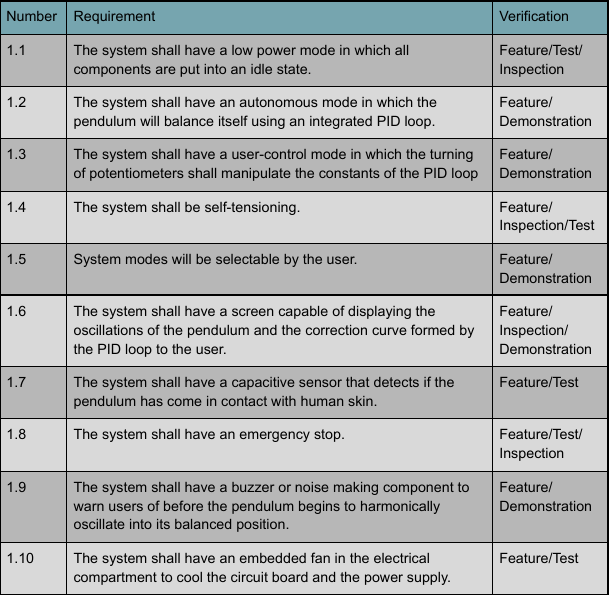
\includegraphics[height=5cm]{FunctionalRequirements}
            \end{block}
        \end{column}

        \begin{column}{0.48\textwidth}
            The functional requirements detail what will make our system, \textbf{our system}. Features
            that are required for us to actually \textbf{solve the problem} we want to solve.
            The most important features include having a \textbf{good user interface mode}, and safety
            systems like an \textbf{emergency stop and guards}.
        \end{column}
    \end{columns}

\note{
\huge Joe \normalsize

\begin{itemize}
 \item Our requirements are the minimums we feel that we need to hit to make our system complete the task it was designed to do
 \item Our most critical system requirements are to have a good user interface and to have saftey sytems like the emergency stop and gaurds.
\end{itemize}
}

\end{frame}

\subsection{Performance Requirements}
\begin{frame}
    \frametitle{Performance Requirements}

    \begin{columns}
        \begin{column}{0.48\textwidth}
            Performance Requirements decide critical performance targets, ie, it should be so
            fast or so quiet or so efficient. The most important in our performance requirements
            are features such as \textbf{Self Starting} and function of the \textbf{Buttons}.
        \end{column}

        \begin{column}{0.48\textwidth}
            \begin{block}{Performance Assessment}
                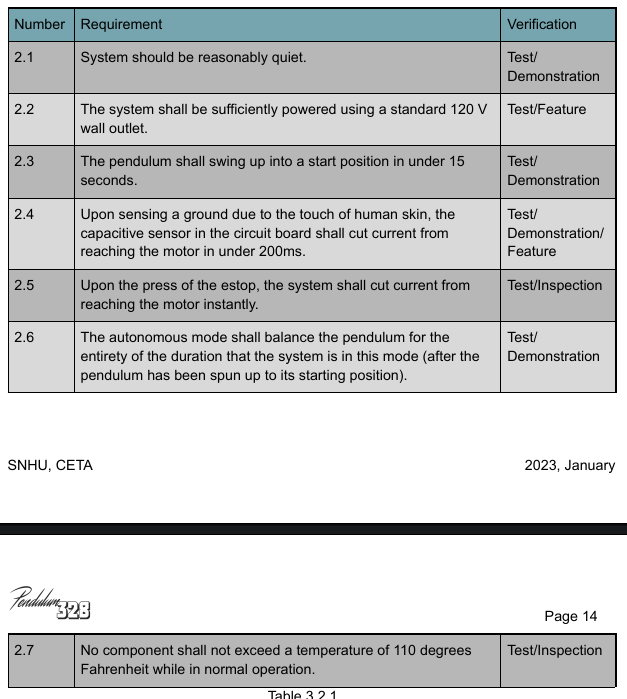
\includegraphics[height=5cm]{PerformanceRequirement}
            \end{block}
        \end{column}
    \end{columns}

\note{
\huge Austin and Matt (Describe a requirement) \normalsize

\begin{itemize}
 \item Our system also has to perform well, and needs certian features such as auto balancing
 \item self starting
 \item and functioning buttons and controls
\end{itemize}
}

\end{frame}

\subsection{Physical Requirement}
\begin{frame}
    \frametitle{Physical Requirements}

    \begin{columns}
        \begin{column}{0.48\textwidth}
            \begin{block}{Physical Requirements}
                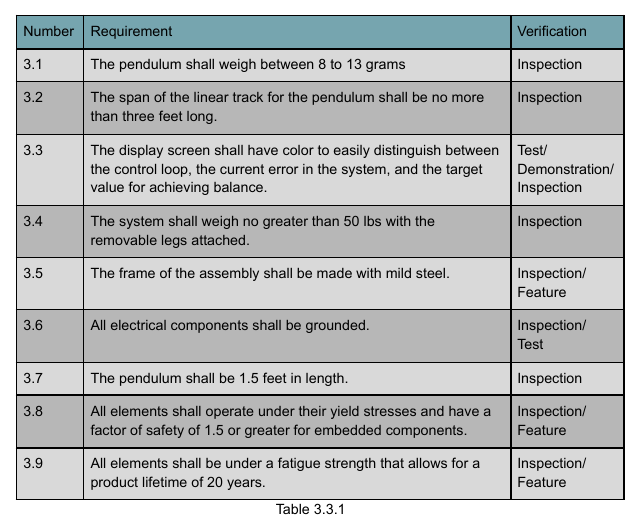
\includegraphics[height=5cm]{PhysicalRequirement}
            \end{block}
        \end{column}

        \begin{column}{0.48\textwidth}
            Physical Requirements are like the other requirements and define the physical
            attributes that define success in solving our product's problem. The most important here
            involve proper use of \textbf{Material} and physical strength requirements.
        \end{column}
    \end{columns}

\note{
\huge Matt and Kat (describes a requirement) \normalsize

\begin{itemize}
 \item There are some phsysical limits to our system as well, it needs to be
 \item made from strong materials
 \item have a long life
 \item and be made from easily replacable, standard components wherever possible
\end{itemize}
}

\end{frame}

\subsection{Risk Assessment}
\begin{frame}
    \frametitle{Risk Assessment}

    \begin{columns}
        \begin{column}{0.48\textwidth}
            Any product or plan comes with risks but mitigation of risks can help make a safe
            and functional product, a couple of the most critical components of our risk assessment
            were safety involving \textbf{Pinch Points}, being \textbf{Struck by moving components}
            or the potential risk of electrical fire due to electronics inside.
        \end{column}

        \begin{column}{0.48\textwidth}
            \begin{block}{Risk Assessment}
                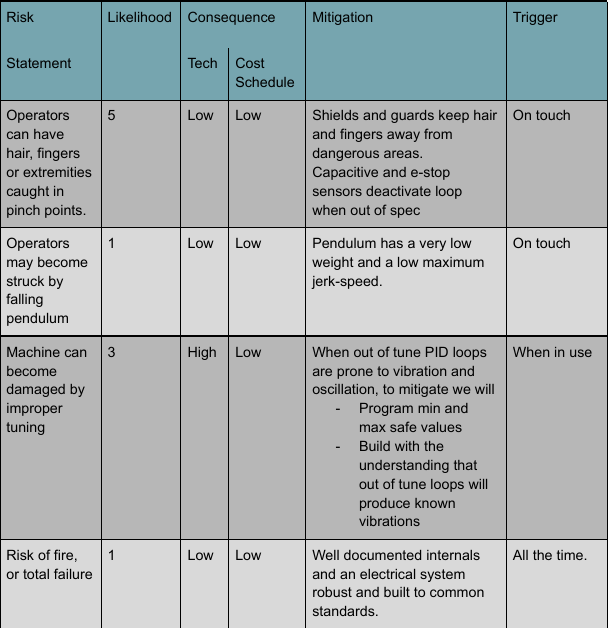
\includegraphics[height=5cm]{RiskAssesment}
            \end{block}
        \end{column}
    \end{columns}

\note{
\huge Joe and Matt (describes requiremnt) \normalsize

\begin{itemize}
 \item Its important to consider the risks when designing a product, some of our most important considerations and \textbf{mitigations} are focused around
 \item Pinch points
 \item Moving parts
 \item Electrical hazzards
 \item and damage to the machine by normal training use.
\end{itemize}

\huge Plz no bonk \normalsize
}

\end{frame}

\subsection{Enviormental Requirements}
\begin{frame}
    \frametitle{Environmental Requirements}

    \begin{columns}
        \begin{column}{0.48\textwidth}
            \begin{block}{Environmental Requirements}
                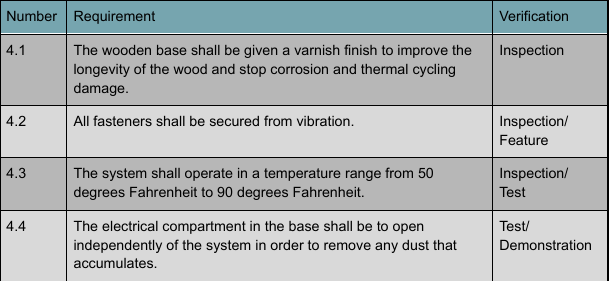
\includegraphics[width=7.3cm]{EnviromentalAndSafety}
            \end{block}
        \end{column}

        \begin{column}{0.48\textwidth}
            We know that our product will be used in some environment, if we want to design a safe
            and functional product we need to take this into account, things like \textbf{Usage schedule}
            and the quality of the air we're blowing over our electronics, mitigation of
            \textbf{dust and oils} as well.
        \end{column}
    \end{columns}

\note{
\huge Kat \normalsize

\begin{itemize}
 \item We expect that our product will be used in some enviorment so we've developed requirements to target the sort of situations we think it will be used in
 \item things like planning for dust ingress, skin oils, normal lubrication and air quality
 \item The system should consider vibrations and effects of long term use
\end{itemize}
}

\end{frame}

\subsection{Engineering Standards}
\begin{frame}
    \frametitle{Engineering Standards}

    \begin{columns}
        \begin{column}{0.48\textwidth}
            Designing to existing engineering standards not only reduces work but makes it easier
            for another team or engineer to make modifications, repairs upgrades or ensure future
            interoperability with existing systems.
        \end{column}

        \begin{column}{0.48\textwidth}
            \begin{block}{Engineering Standards}
                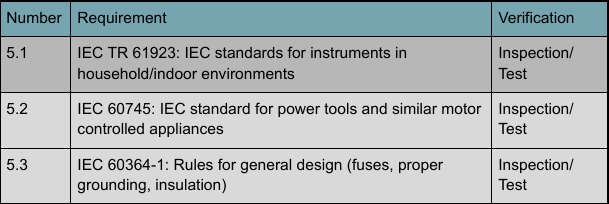
\includegraphics[width=7.3cm]{EngineeringStandards}
            \end{block}
        \end{column}
    \end{columns}

\note{
\huge Joe's got this one \normalsize

\begin{itemize}
 \item Building to existing engineering standards reduces our workload,
 \item promotes easier servicing in situ,
 \item and makes our product safer by following established guidelines
\end{itemize}
}

\end{frame}

\section{Design Concepts}
\begin{frame}
    \frametitle{Design Concepts (1)}

    \begin{columns}
        \begin{column}{0.48\textwidth}
            \begin{block}{Sketch 1}
                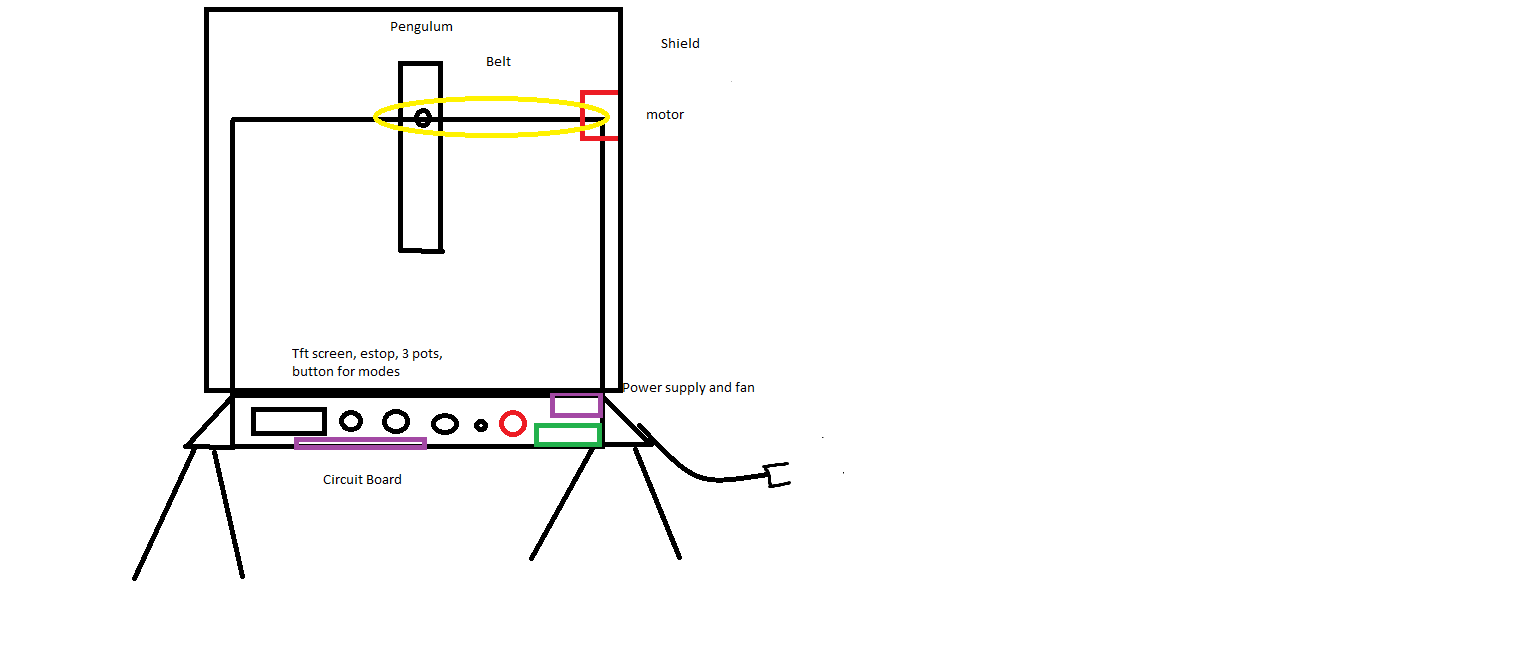
\includegraphics[height=6cm]{../../../Notes/Sketches/Basic Mock-Up Sketch.png}
            \end{block}
        \end{column}

        \begin{column}{0.48\textwidth}
            \begin{block}{Sketch 2}
                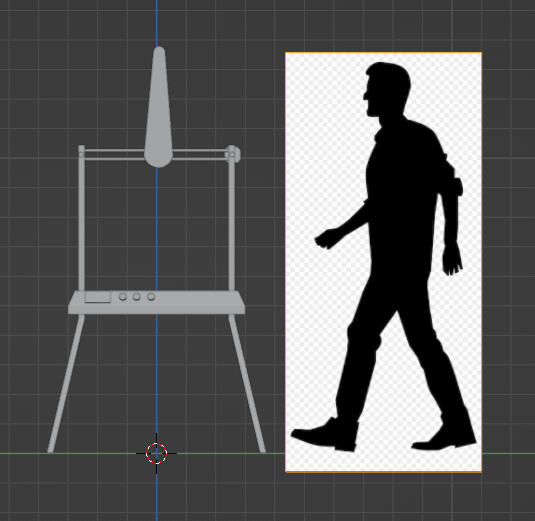
\includegraphics[height=6cm]{Scale}
            \end{block}
        \end{column}
    \end{columns}

\note{
\begin{itemize}
 \item Sketch 1 is our inital design concept drawn by Matt <3
 \item Sketch 2 shows how our product may look sizewise compared to a 5'11" person
\end{itemize}
}

\end{frame}

\begin{frame}
    \frametitle{Design Concepts (2)}

    \begin{columns}
        \begin{column}{0.48\textwidth}
            \begin{block}{Sketch 3}
                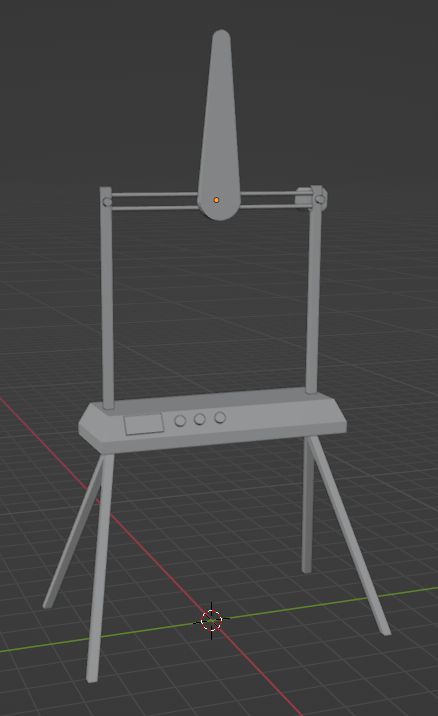
\includegraphics[height=6cm]{Full}
            \end{block}
        \end{column}

        \begin{column}{0.48\textwidth}
            \begin{block}{Sketch 4}
                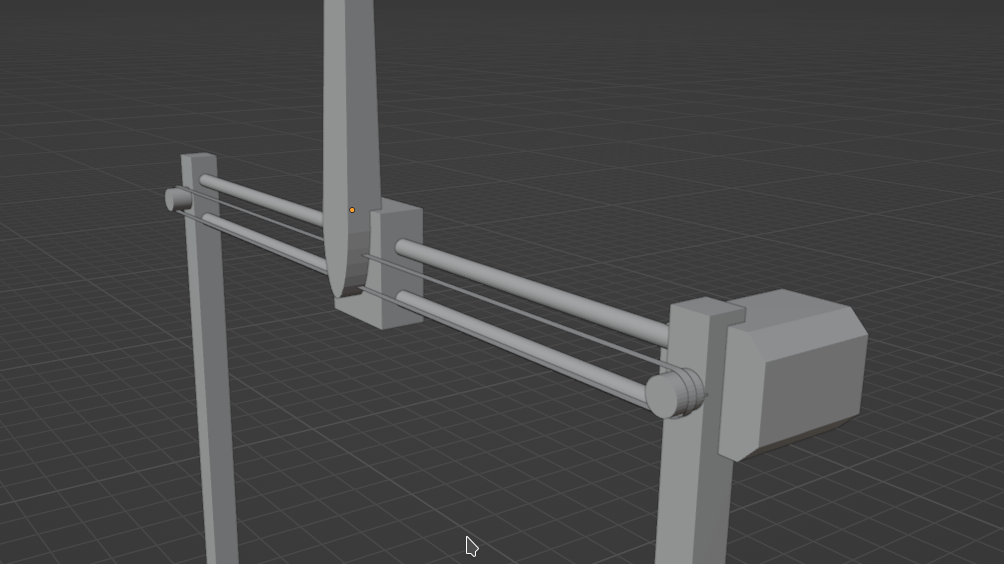
\includegraphics[width=7.3cm]{UpperAssy}
            \end{block}
        \end{column}
    \end{columns}

\note{
\begin{itemize}
 \item Sketch 3 is another view of our inital 3d model
 \item and sketch 4 shows what our motor and trolley carriage may look like with belt between them
\end{itemize}
}

\end{frame}

\begin{frame}
    \frametitle{Design Concepts (3)}

    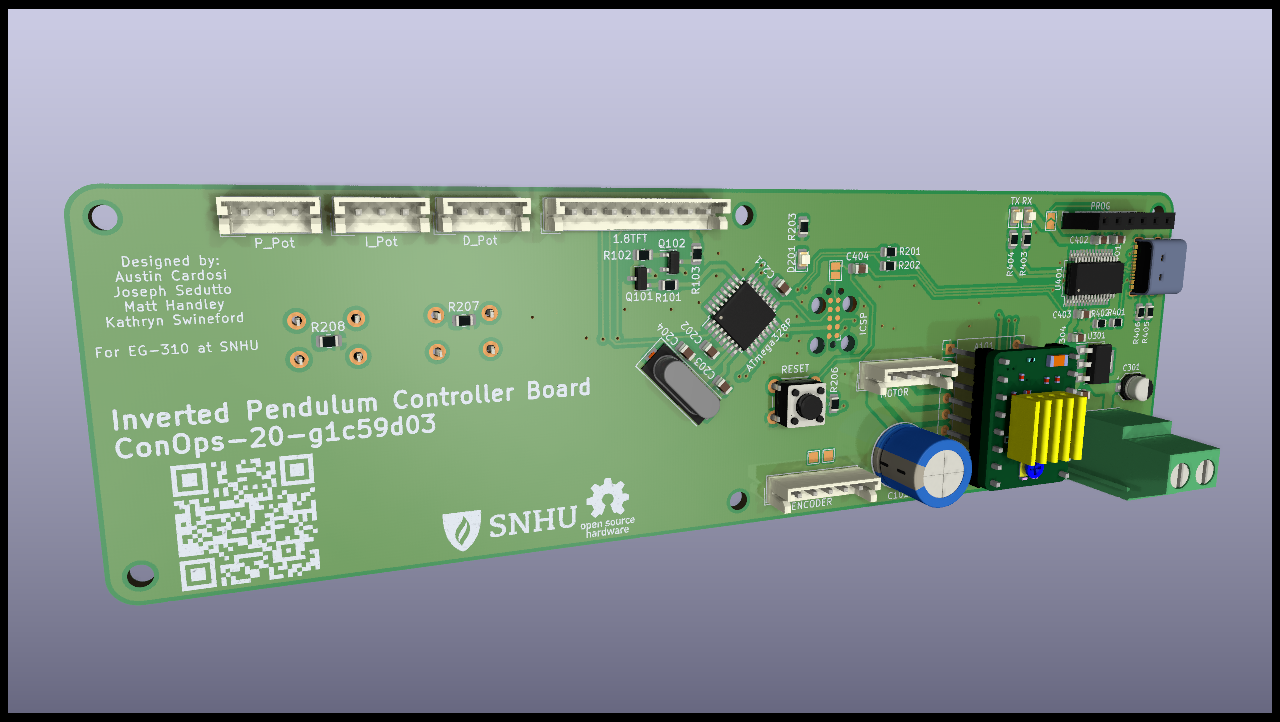
\includegraphics[width=10cm]{CircuitBoard}

\note{
\begin{itemize}
 \item We're nearing completion with our controller board.
\end{itemize}
}

\end{frame}

\begin{frame}
    \frametitle{Design Concepts (4)}

    \begin{columns}
        \begin{column}{0.48\textwidth}
            \begin{block}{Sketch 5}
                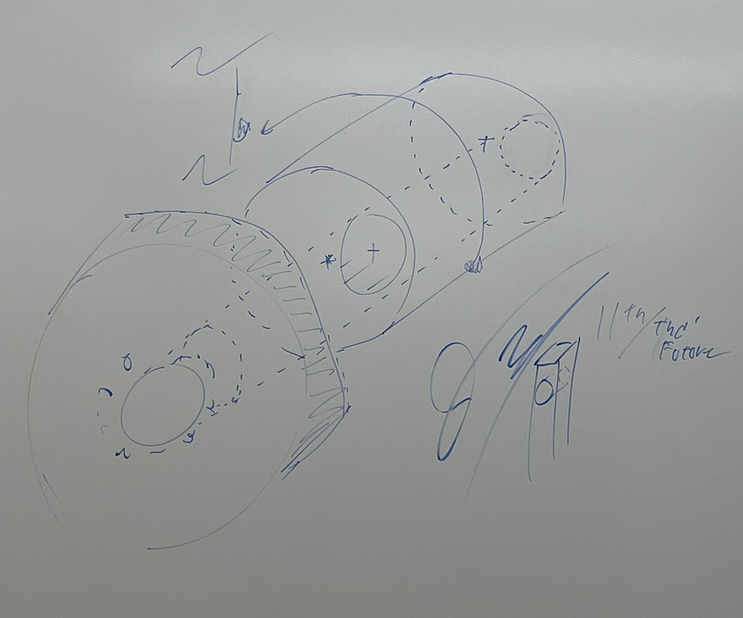
\includegraphics[height=6cm]{Tension}
            \end{block}
        \end{column}

        \begin{column}{0.32\textwidth}
            \begin{block}{Sketch 6}
                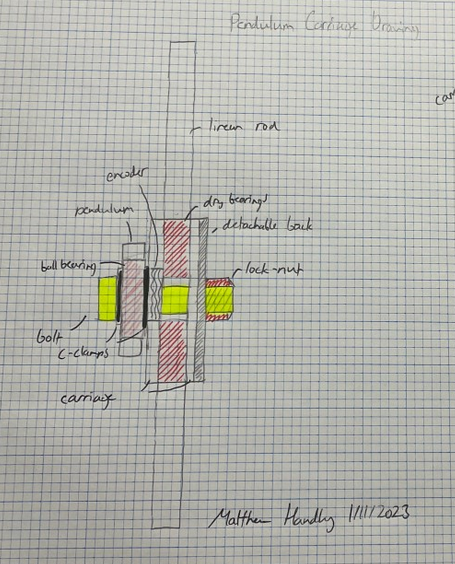
\includegraphics[height=6cm]{Carriage}
            \end{block}
        \end{column}
    \end{columns}

\note{
\begin{itemize}
 \item Some more design concepts, on the left, a common cam-based belt tensioning method that reduces need to service the belt,
 \item on the right we have the bearing stackup for our carriage.
\end{itemize}
}

\end{frame}

\begin{frame}
    \frametitle{Task Plan}

    With both ProjectLibre (An open source program)

    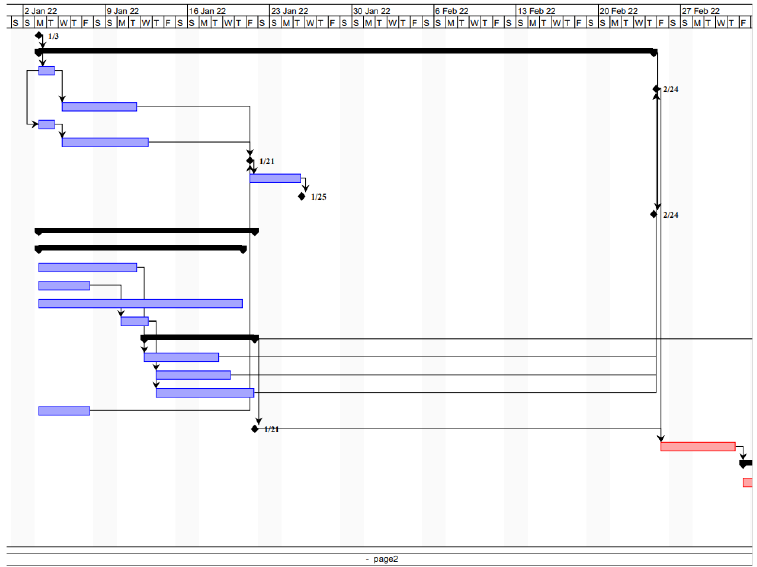
\includegraphics[height=3cm]{ProjectLibre}

    and github task management, we plan and manage our team's productivity.

    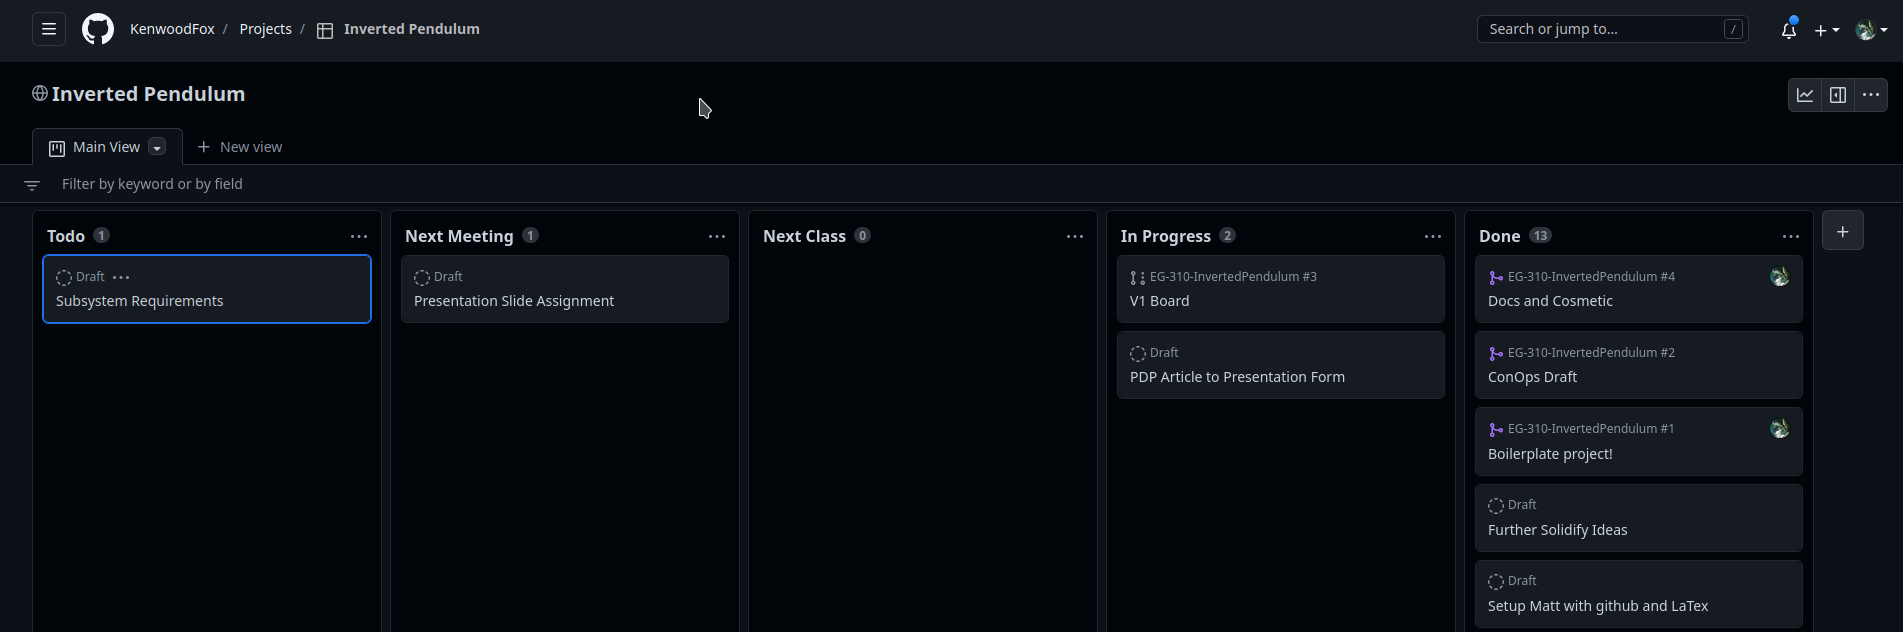
\includegraphics[width=10cm]{ProjectPlan}

\note{
\huge Kat

its a spreadsheet with time slots \normalsize

\begin{itemize}
 \item We plan everything using ProjectLibre and github task management, Theres a larger copy of our ProjectLibre timeline at the end of the presentation.
\end{itemize}
}

\end{frame}

\section{Budget}
\begin{frame}
    \frametitle{Budget}

    \begin{columns}
        \begin{column}{0.70\textwidth}
            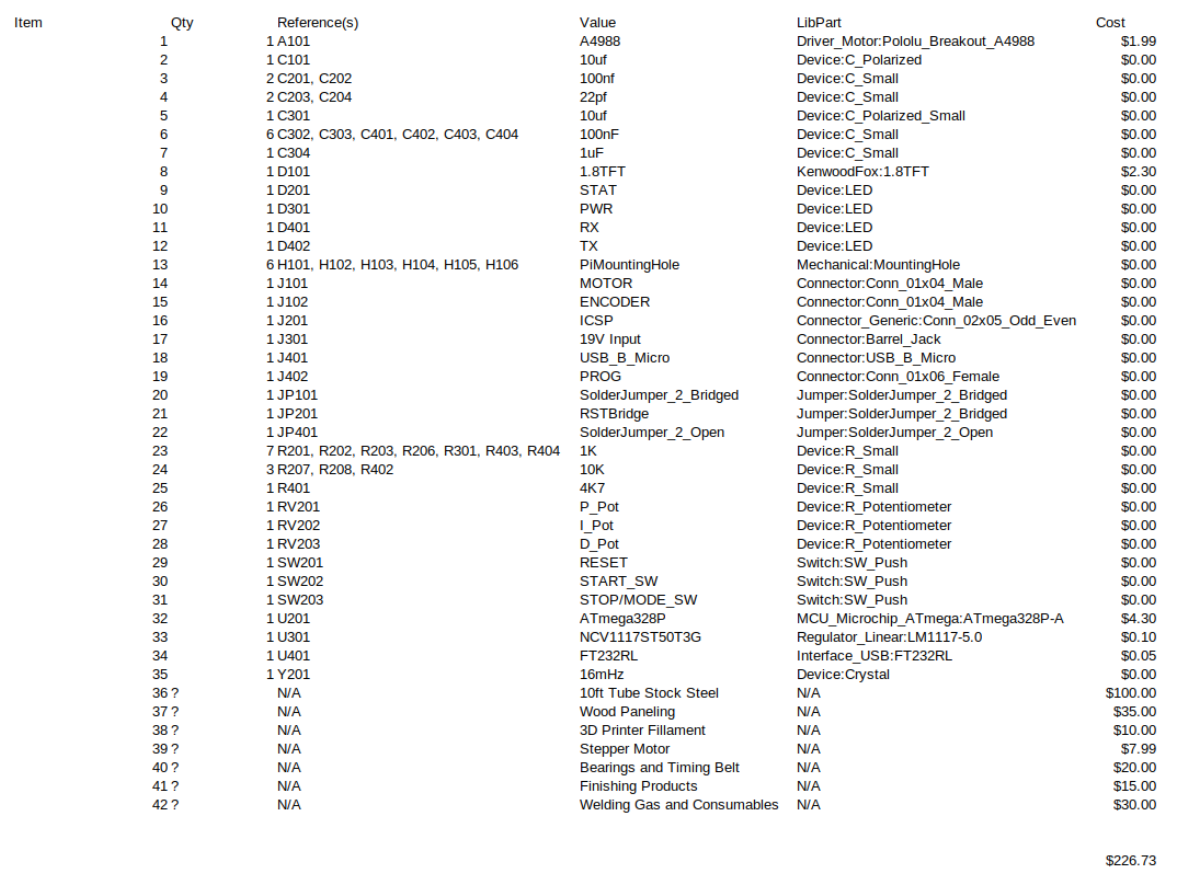
\includegraphics[height=7cm]{BOMTable}
        \end{column}

        \begin{column}{0.30\textwidth}
            We project to complete our project underbudget! With a low upfront development cost.
            We currently project spending \$250 to \$300 for our prototype.
        \end{column}
    \end{columns}

\note{
\huge Austin \normalsize

\begin{itemize}
 \item So far we project we'll be underbudget, between \$250 and \$300
\end{itemize}
}

\end{frame}

\section{Diagrams}
\subsection{Block Diagrams}
\begin{frame}
    \frametitle{Block Diagram}

    \begin{columns}
        \begin{column}{0.70\textwidth}
            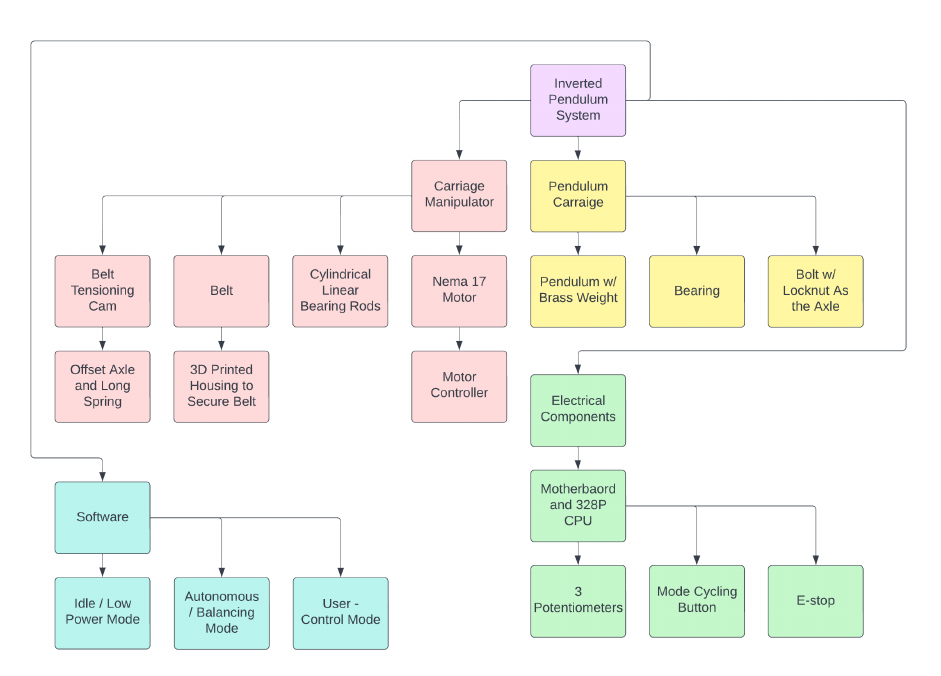
\includegraphics[height=7cm]{BlockDiagram}
        \end{column}

        \begin{column}{0.30\textwidth}
            \begin{block}{Block Diagram}
                The block diagram details the electrical, mechanical and software components.
                And their relationship to each other.
            \end{block}
        \end{column}
    \end{columns}

\note{
\huge Matt \normalsize

\begin{itemize}
 \item Our block diagram shows how our software, hardware and electronics may interact in a final system
\end{itemize}
}

\end{frame}

\subsection{Operations}
\begin{frame}
    \frametitle{Operations}

    \begin{columns}
        \begin{column}{0.30\textwidth}
            \begin{block}{Operations}
                The Operations diagram details the physical and general controls.
            \end{block}
        \end{column}

        \begin{column}{0.70\textwidth}
            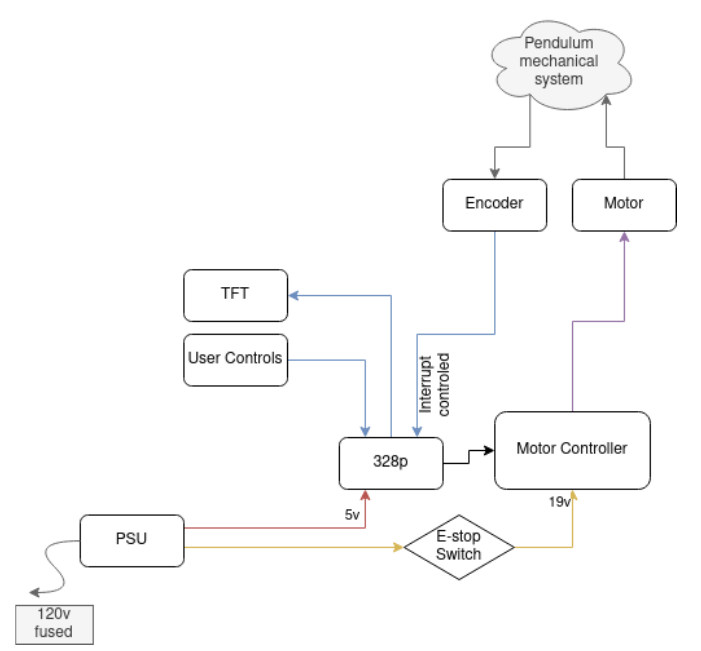
\includegraphics[height=7cm]{Operations}
        \end{column}
    \end{columns}

\note{
\huge Joe \normalsize

\begin{itemize}
 \item The operations chart details our physical and general controls like the tft screen
 \item the buttons
 \item the motor controller and encoders
\end{itemize}
}

\end{frame}

\subsection{Software}
\begin{frame}
    \frametitle{Software Flowchart}

    \begin{columns}
        \begin{column}{0.72\textwidth}
            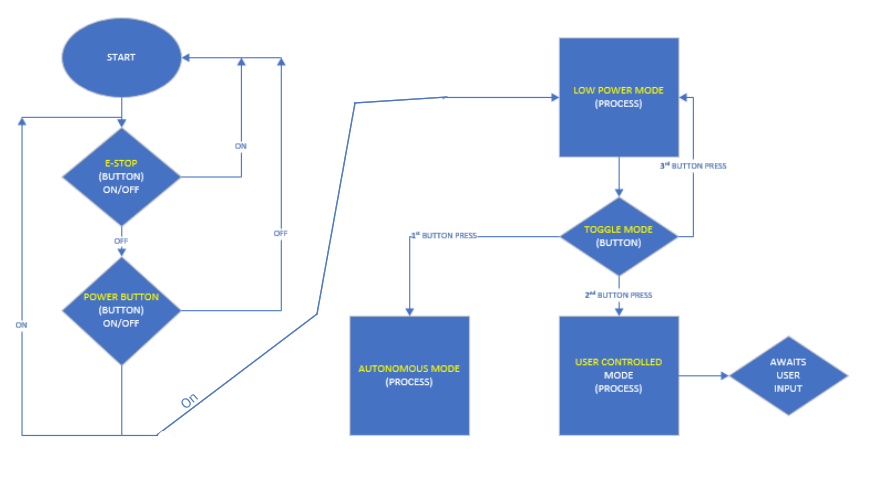
\includegraphics[width=11cm]{SoftwareFlowchart}
        \end{column}

        \begin{column}{0.28\textwidth}
            \begin{block}{Software Flowchart}
                The software flowchart is an overview of all the software functions of our
                proposed product.
            \end{block}
        \end{column}
    \end{columns}

\note{
\huge Austin \normalsize

\begin{itemize}
 \item Our software flowchart details how the PID control scheme will be interactable by the users
\end{itemize}
}

\end{frame}

\section{End}
\begin{frame}
    \frametitle{End}

    \begin{block}{}
        \begin{center}
            \Huge Questions and Comments?
        \end{center}
    \end{block}

    \begin{center}
        Find the source code for this document, and the rest of our designs, firmware, hardware
        and notes on GitHub!

        
\includegraphics[height=2cm]{github_qr}
    \end{center}

\note{
\begin{itemize}
 \item So please if you have any questions we would love to hear them.
 \item All of our software, CAD, hardware and design docs are licensed under
 \item \huge The MIT Open Source License \normalsize and available via git.
 \item If you have a specific slide in mind we can go back to it!
\end{itemize}
}

\end{frame}

\section{Appendices}
\begin{frame}
    \frametitle{References}

    \includegraphics[height=4cm]{references}
\end{frame}

\begin{frame}
    \frametitle{Complete Timeline}

    \includegraphics[width=15cm]{project}
\end{frame}

\begin{frame}
    \frametitle{Calculations}

    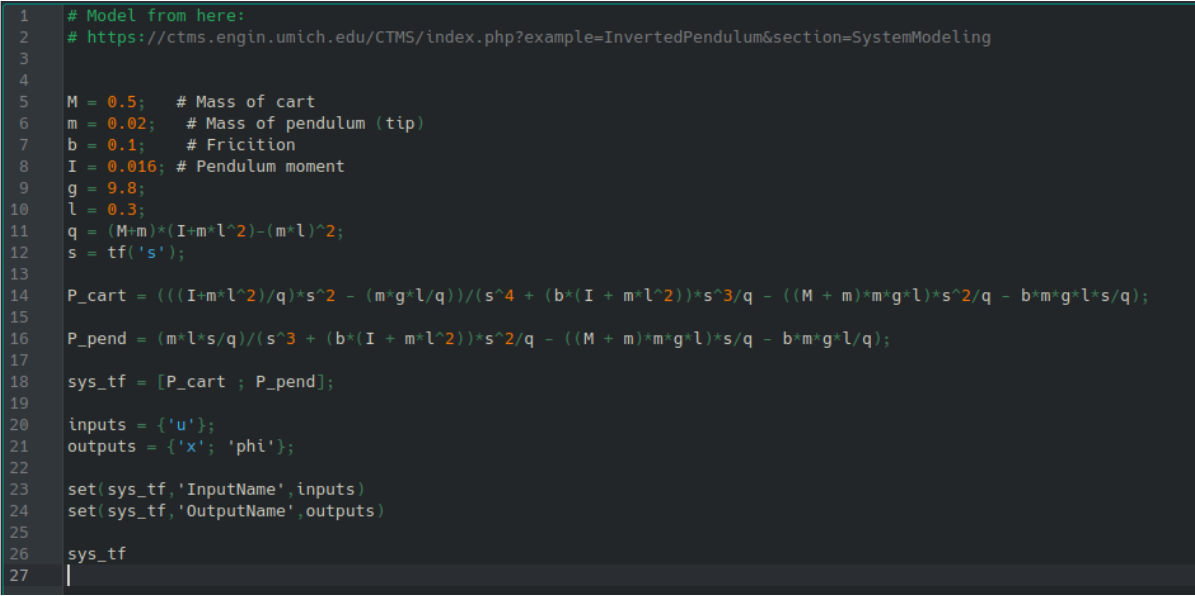
\includegraphics[height=6.5cm]{Calculations}

    Octave math model.
\end{frame}


\end{document}
